%*******************************************************%
%														%
% William Cunningham									%
% wcunning@umich.edu									%
% EECS 470 -- Lab 2										%
%														%
%*******************************************************%

%*******************************************************%
% Preamble												%
%*******************************************************%

\documentclass[table,dvipsnames]{beamer}
\usetheme{Lab}

\usepackage{
	siunitx,
	tikz,
	graphicx,
	amsmath,
	float,
	minted,
	hyperref,
	textcomp,
	upquote,
	multirow,
	fancyvrb
}

\usepackage[T1]{fontenc}
%-----------------------%
% TikZ					%
%-----------------------%
%--- CircuiTikZ Definitions ---%

%--- TikZ Definitions ---%
\usetikzlibrary{shapes,arrows,automata,shadows,decorations,fadings}
\pgfdeclarelayer{background}
\pgfdeclarelayer{foreground}
\pgfsetlayers{background,main,foreground}
\tikzstyle{master-blank} = 
[	draw, 
	rounded corners, 
	rectangle,
	color=ForestGreen!25,
	minimum height=0.5cm, 
	minimum width=1.30cm
]
\tikzstyle{master-commit} = 
[	draw, 
	fill=ForestGreen!50, 
	rounded corners, 
	rectangle,
	minimum height=0.5cm, 
	minimum width=1.30cm
]
\tikzstyle{branch-commit} = 
[	draw, 
	fill=RoyalBlue!70, 
	rounded corners,
	rectangle,
	minimum height=0.5cm, 
	minimum width=1.30cm
]
\tikzstyle{clean-repo} = 
[	draw, 
	inner color=RoyalBlue!40, 
	outer color=RoyalBlue!50, 
	color=black,
	circle,
	minimum height=2cm
]
\tikzstyle{changes-repo} = 
[	draw, 
	inner color=Red!40, 
	outer color=Red!50, 
	color=black,
	circle,
	minimum height=2cm
]

\definecolor{darkblue}{rgb}{0,0,0.8}

\hypersetup{colorlinks=true,linkcolor=,urlcolor=red}

\newcommand{\masterrepo}[2]{
	\scriptsize{\color{Black}\texttt{#1}} \\
	\scriptsize{\color{OliveGreen}\texttt{HEAD=#2}}
}

\newcommand{\branchrepo}[2]{
	\scriptsize{\color{Black}\texttt{#1}} \\
	\scriptsize{\color{NavyBlue}\texttt{HEAD=#2}}
}

\newcommand{\commit}[1]{
	\scriptsize{\texttt{#1}}
}

%*******************************************************%
% Document												%
%*******************************************************%

\title[Lab 4: VCS]{EECS 470 Lab 4}
\subtitle{Version Control System}
\institute[University of Michigan]{Department of Electrical Engineering and 
			Computer Science \\
			College of Engineering \\
			University of Michigan}
<<<<<<< HEAD
\date{Thursday, 31$^{\text{st}}$ January, 2019}
=======
\date{Thursday, 26$^{\text{st}}$ September, 2019}
>>>>>>> 2618214ed0a9931a8b9fe8e5baf7fe250a614812

\begin{document}
\frame{\titlepage}

\begin{frame}{Overview}
	\tableofcontents
\end{frame}

\section{Administrivia}
\begin{frame}{Administrivia}
	\begin{block}{Homework}
		\begin{itemize}
			\item Homework 2 is due Thursday, 31$^{\text{st}}$ February at 11:59PM
			\item If you haven't, you need to get started \emph{now}
		\end{itemize}
	\end{block}
	\begin{block}{Projects}
		\begin{itemize}
			\item Project 3 is due on Monday, 7$^{\text{th}}$ October at midnight
		\end{itemize}
	\end{block}
	\begin{block}{}
		We are available to answer questions on anything here. Office hours can
		be found in the
		%\href{https://www.google.com/calendar/embed?src=tcmcrdofi69t5bunjo01onoi1s\%40group.calendar.google.com}{course google calendar}
		course website.
	\end{block}
\end{frame}

\section{Git}
\subsection{VCS Basics}
\begin{frame}{Version Control Systems}
	\begin{block}{What is a version control system?}
		\begin{itemize}
			\item Stores text files
			\item Keeps old versions around
			\item Allows parallel work
		\end{itemize}
	\end{block}
	\begin{block}{Why do I care?}
		\begin{itemize}
			\item Prevents/helps prevent loss of data (nothing is foolproof)
			\item Great for group work
			\item Required for Project 3
		\end{itemize}
	\end{block}
\end{frame}

\begin{frame}{History of VCS}
	\begin{block}{Motivation}
		Avoid having
		\begin{itemize}
			\item \texttt{isr.v.old}
			\item \texttt{isr.v.old2}
			\item \texttt{isr.v.working}
			\item \texttt{isr.v.REALLY\_working}
		\end{itemize}
	\end{block}
	\begin{block}{A Short History}
		\begin{tabular}{lll}
			\rowcolor{RoyalBlue!50}
			1950 & Manual file naming			& \\ 
			\rowcolor{RoyalBlue!50}
			1982 & Revision Control System		& \multirow{-2}{*}{Local} \\ 
			\rowcolor{RoyalBlue!25}
			1986 & Concurrent Versions System	& \\
			\rowcolor{RoyalBlue!25}
			2000 & Subversion					& \multirow{-2}{*}{Central} \\ 
			\rowcolor{RoyalBlue!50}
			2005 & Git							& Distributed \\ 
		\end{tabular}
	\end{block}
\end{frame}

\subsection{Distributed VCS}
\begin{frame}<0>[label=dvcs]{Distributed VCS}
	\begin{figure}[H]
		\centering
		\begin{tikzpicture}[auto, node distance=1.5cm,>=latex',every text node part/.style={align=center}]
			\def\blockdist{1cm}
			\def\edgedist{1cm}

			\begin{pgfonlayer}{foreground}
				%--[ Server ]--%
				\node<2->[
					clean-repo,
					align=center
					] 
					(server) 
					{};
				%--[ Brehob ]--%
				\node[
					clean-repo,
					xshift=-2.35cm,
					yshift=-3cm
					] 
					(brehob)
					{};
				\draw<2->[
					very thick,
					<->
					] 
					(brehob.north) .. controls+(90:0.75cm) and +(255:0.75cm) .. (server.south west);
				%--[ Jon ]--%
				\node[
					clean-repo,
					xshift=0cm,
					yshift=-3cm
					]
					(jon)
					{};
				\draw<2->[
					very thick,
					<->
					]
					(jon.north) -- (server.south);
				%--[ Will ]--%,13-15,18->{
				\node[
					clean-repo,
					xshift=2.35cm,
					yshift=-3cm
					] 
					(will)
					{};
				\draw<2->[
					very thick,
					<->
					] 
					(will.north) .. controls+(90:0.75cm) and +(285:0.75cm) .. (server.south east);
				\draw<1>[very thick,<->] (will.105) to[bend right] (jon.75);
				\draw<3>[very thick,red,<->] (will.105) to[bend right] (jon.75);
				\draw<1>[very thick,<->] (brehob.75) to[bend left] (jon.105);
				\draw<3>[very thick,red,<->] (brehob.75) to[bend left] (jon.105);
				\draw<1>[very thick,<->] (brehob.270) to[bend right] (will.270);
				\draw<3>[very thick,red,<->] (brehob.270) to[bend right] (will.270);
			\end{pgfonlayer}
			\begin{pgfonlayer}{background}
				\only<1>{
					\path (brehob.north -| brehob.west)+(-0.5cm,1cm) node (a) {};
				}
				\only<2->{
					\path (server.north -| brehob.west)+(-0.5cm,1cm) node (a) {};
				}
				\path (will.east |- will.south)+(0.5cm,-0.9cm) node (b) {};
				\path[fill=Cerulean!25, rounded corners, draw=black!50, dashed] (a) rectangle (b);
	
				\node[above of=server,yshift=0cm] () {\Large{VCS
					Structure --
					\only<2>{Centralized}\only<1>{Distributed}\only<3>{Hybrid}}};
			\end{pgfonlayer}
		\end{tikzpicture}
	\end{figure}
\end{frame}

\begin{frame}{Centralized VCS}
	\begin{block}{What does it mean to be centralized?}
		\begin{itemize}
			\item Clients talk to a server, which is the one, true version
			\item Server copy keeps history
			\item Clients have a(n) (incomplete) \emph{working copy}
		\end{itemize}
	\end{block}
\end{frame}

\againframe<2>{dvcs}

\begin{frame}{Distributed VCS}
	\begin{block}{What does it mean to be distributed?}
		\begin{itemize}
			\item Every copy is created equal (can all act as the server)
			\item No one, true version
		\end{itemize}
	\end{block}
\end{frame}

\againframe<1>{dvcs}

\begin{frame}{Hybrid VCS}
	\begin{block}{The Hybrid Approach}
		\begin{itemize}
			\item Use a DVCS
			\item Set up a server to be the synchronization point
			\item Possibly still connect directly to colleagues, but generally
				not
		\end{itemize}
	\end{block}
\end{frame}

\againframe<3>{dvcs}

\subsection{Git Preliminaries}
\frame{\subsectionpage}
\begin{frame}{Secure Shell}
	\begin{block}{What is \texttt{ssh}?}
		\begin{itemize}
			\item Secured remote connection to a server, e.g.
				\begin{itemize}
					\item Remote shell
					\item How git (should) communicate(s) with other machines 
				\end{itemize}
		\end{itemize}
	\end{block}
	\begin{block}{What do I need to know?}
		\begin{itemize}
			\item Requires that you identify yourself:
				\begin{itemize}
					\item Key (RSA or DSA)
					\item Password (keyboard-interactive)
					\item Kerberos (gssapi-with-mic)
				\end{itemize}
			\item Necessary for Bitbucket (coming up)
		\end{itemize}
	\end{block}
\end{frame}

\begin{frame}{Secure Shell: Keys}
	\begin{block}{SSH Keys}
		\begin{itemize}
			\item Public-private key pair authentication
			\item Can also be password protected
		\end{itemize}
	\end{block}
	\begin{block}{\texttt{ssh-keygen}}
		\begin{itemize}
			\item Creates \texttt{\~{}/.ssh/id\_rsa} (your private key) and
				\texttt{\~{}/.ssh/id\_rsa.pub} (your public key)
		\end{itemize}
	\end{block}
\end{frame}

\begin{frame}{Example: \texttt{ssh-keygen}}
	\VerbatimInput[fontsize=\scriptsize,frame=single]{ssh-keygen.txt}
\end{frame}

\begin{frame}{Git Configuration}
	\begin{block}{Follow Along}
		\begin{itemize}
			\item Run the following commands:
				\begin{itemize}
					\item \texttt{git config -{}-global user.name ``Your Name''}
					\item \texttt{git config -{}-global user.email ``uniqname@umich.edu''}
				\end{itemize}
% 			\item Optionally:
% 				\begin{itemize}
% 					\item Download
% 						\href{http://www-personal.umich.edu/~wcunning/wcunning-dotfiles.tar.gz}{wcunning-dotfiles.tar.gz}
% 					\item Open it up
% 					\item Copy \texttt{.gitconfig} and \texttt{.gitignore} to
% 						your home directory
% 					\item Optionally copy other configs/google those programs
% 				\end{itemize}
		\end{itemize}
	\end{block}
\end{frame}

\begin{frame}[fragile]{Bitbucket}
	\begin{block}{What is \href{https://bitbucket.org/}{Bitbucket}?}
		\begin{itemize}
			\item Free, online git repositories
			\item More friendly to private repos than Github
		\end{itemize}
	\end{block}
	\begin{block}{What do I need to know?}
		\begin{itemize}
			\item Used for Project 3 and the final project
			\item You need to make an account, right now
			\item Once you have an account, add it to this
				\href{https://docs.google.com/spreadsheets/d/1N5EKp01RqMQF2hDmvTimF4kjQmUhuaGxmFt1uVJ_rUI/edit?usp=sharing}{spreadsheet}
		\end{itemize}
	\end{block}
	\hyperlink{bitbucket}{\beamergotobutton{How to make a Bitbucket account\dots}}
\end{frame}

\subsection{Git Basics by Example}

\begin{frame}{Example Execution}
	\VerbatimInput[fontsize=\tiny,frame=single]{example.txt}
\end{frame}


\begin{frame}{Git Basics Introduction}
	\begin{block}{Structure}
		For each command you need to know, we will
		\begin{enumerate}
			\item Occasionally, an aside with a Git Concept we need to describe
				a command
			\item Describe the command, along with any useful flags/options
			\item Show how the command affects the repositories
			\item Show an example with output
		\end{enumerate}
	\end{block}
\end{frame}

\begin{frame}{Git Diagram}
	\vspace*{-24pt}
	\begin{columns}
		\hspace*{-0.075\textwidth}
		\begin{column}[T]{0.6\textwidth}
			\begin{figure}[H]
				\centering
				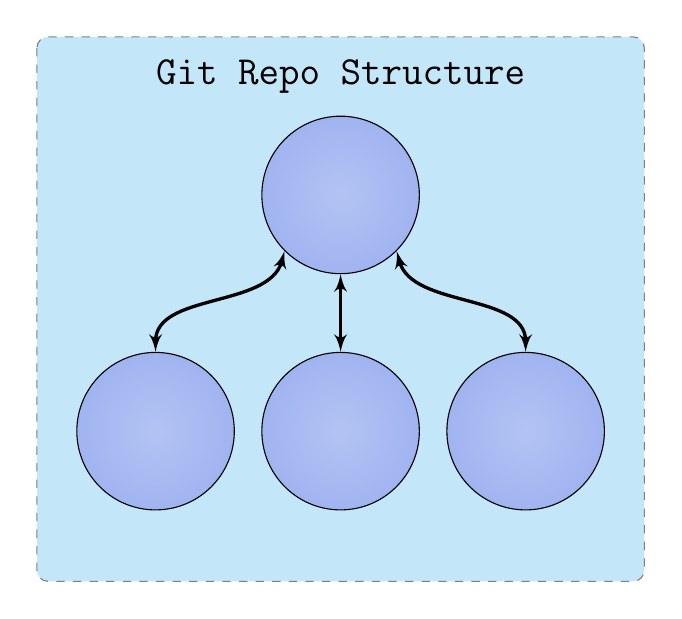
\begin{tikzpicture}[auto, node distance=1.5cm,>=latex',every text node part/.style={align=center}]
					\def\blockdist{1cm}
					\def\edgedist{1cm}

					\begin{pgfonlayer}{foreground}
						%--[ Server ]--%
						\node[
							clean-repo,
							align=center
							] 
							(server) 
							{};
						%--[ Brehob ]--%
						\node[
							clean-repo,
							xshift=-2.35cm,
							yshift=-3cm
							] 
							(brehob)
							{};
						\draw[
							very thick,
							<->
							] 
							(brehob.north) .. controls+(90:0.75cm) and +(255:0.75cm) .. (server.south west);
						%--[ Jon ]--%
						\node[
							clean-repo,
							xshift=0cm,
							yshift=-3cm
							]
							(jon)
							{};
						\draw[
							very thick,
							<->
							]
							(jon.north) -- (server.south);
						%--[ Will ]--%,13-15,18->{
						\node[
							clean-repo,
							xshift=2.35cm,
							yshift=-3cm
							] 
							(will)
							{};
						\draw[
							very thick,
							<->
							] 
							(will.north) .. controls+(90:0.75cm) and +(285:0.75cm) .. (server.south east);
					\end{pgfonlayer}
					\begin{pgfonlayer}{background}
						\path (server.north -| brehob.west)+(-0.5cm,1cm) node (a) {};
						\path (will.east |- will.south)+(0.5cm,-0.9cm) node (b) {};
						\path[fill=Cerulean!25, rounded corners, draw=black!50, dashed] (a) rectangle (b);
			
						\node[above of=server,yshift=0cm] () {\Large{\texttt{Git Repo
						Structure}}};
					\end{pgfonlayer}
				\end{tikzpicture}
			\end{figure}
		\end{column}
		\begin{column}[T]{0.25\textwidth}
			\begin{figure}[H]
				\centering
				\begin{tikzpicture}[auto, node distance=1.25cm,>=latex',every text node
					part/.style={align=center}]
					\def\blockdist{1cm}
					\def\edgedist{1cm}

					\begin{pgfonlayer}{foreground}
						\node[master-commit] (HEAD4) {\commit{9a12490}};
						\draw[very thick,color=OliveGreen!50,dashed,->] (HEAD4)+(0,-1cm) -- (HEAD4.south);
						\node[master-blank,above of=HEAD4] (HEAD3) {};
						\node[master-blank,above of=HEAD3] (HEAD2) {};
						\node[master-blank,above of=HEAD2] (HEAD1) {};
						\node[master-blank,above of=HEAD1] (HEAD) {};
						
						\only<26->{
							\node[
								%master-blank,
								left of=HEAD,
								node distance=1.50cm,
								yshift=0cm
								] 
								(tag) 
								{\alert{\texttt{lab4}}};
							\draw[
								very thick,
								color=Red,
								->
							] (tag) -- (HEAD);
						}
						
						\only<-23>{
							\node[
								master-blank,
								left of=HEAD1,
								node distance=1.45cm,
								yshift=0cm
								] 
								(BR) 
								{};
						}
						\only<23->{
							\node[
								branch-commit,
								left of=HEAD1,
								node distance=1.45cm,
								yshift=0cm
								] 
								(BR) 
								{\commit{06505f6}};
							\draw[very thick,color=NavyBlue!75!black,->] (BR1.north) -- (BR.south);
						}
						\only<-13>{
							\node[
								master-blank,
								left of=HEAD2,
								node distance=1.45cm,
								yshift=0cm
								] 
								(BR1) 
								{};
						}
						\only<13->{
							\node[
								branch-commit,
								left of=HEAD2,
								node distance=1.45cm,
								yshift=0cm
								] 
								(BR1)
								{\commit{8e4bab6}};
						}

						\only<25->{
							\draw[very thick,color=NavyBlue!75!black,->] (BR.north) ..
							controls+(90:0.75cm) and +(270:0.5cm) .. (HEAD.south);
						}
						\only<10->{
							\draw[very thick,color=NavyBlue!75!black,->] (HEAD3.north) ..
							controls+(90:0.5cm) and +(270:0.75cm) .. (BR1.south);
						}
					\end{pgfonlayer}
					\begin{pgfonlayer}{background}
						\path (HEAD.north -| BR.west)+(-0.5cm,1cm) node (a) {};
						\path (HEAD.east |- HEAD4.south)+(0.5cm,-0.5cm) node (b) {};
						\path[fill=ForestGreen!25, rounded corners, draw=black!50, dashed] (a) rectangle (b);

						\node[above of=HEAD,yshift=-0.5cm,xshift=-0.625cm] () {\texttt{\Large{Commit Tree}}};
					\end{pgfonlayer}
				\end{tikzpicture}
			\end{figure}
		\end{column}
	\end{columns}
\end{frame}
\begin{frame}<1>[label=diagram]{Git Diagram}
	\vspace*{-24pt}
	\begin{columns}
		\hspace*{-0.075\textwidth}
		\begin{column}[T]{0.6\textwidth}
			\begin{figure}[H]
				\begin{tikzpicture}[auto, node distance=1.5cm,>=latex',every text node part/.style={align=center}]
					\def\blockdist{1cm}
					\def\edgedist{1cm}

					\begin{pgfonlayer}{foreground}
						%--[ Server ]--%
						\node[
							clean-repo,
							align=center
							] 
							(server) 
							{\masterrepo{[origin]}{\only<1-5>{9a12490}\only<6-19>{f2ea0f5}\only<20->{4b3d3cb}}
							};
						%--[ Brehob ]--%
						\only<1-13,16,19->{
							\node[
								clean-repo,
								xshift=-2.35cm,
								yshift=-3cm
								] 
								(brehob)
								{\masterrepo{Mark}{\only<1-6>{9a12490}\only<7-15>{f2ea0f5}\only<16-18>{b73416d}\only<19->{4b3d3cb}}};
						}
						\only<14-15,17-18>{
							\node[
								changes-repo,
								xshift=-2.35cm,
								yshift=-3cm
								] 
								(brehob)
								{\masterrepo{Mark\only<14,17>{\alert{*}}\only<15,18>{\alert{+}}}
									{\only<1-6>{9a12490}\only<7-15>{f2ea0f5}\only<16-18>{b73416d}\only<19->{4b3d3cb}}
								};
						}
						\only<1-6,8-19,21->{
							\draw[
								very thick,
								%->
								] 
								(brehob.north) .. controls+(90:0.75cm) and +(255:0.75cm) .. (server.south west);
						}
						\only<7>{
							\draw[
								very thick,
								color=Red,
								<-
								] 
								(brehob.north) .. controls+(90:0.75cm) and +(255:0.75cm) .. (server.south west);
						}
						\only<20>{
							\draw[
								very thick,
								color=Red,
								->
								] 
								(brehob.north) .. controls+(90:0.75cm) and +(255:0.75cm) .. (server.south west);
						}
						%--[ Jon ]--%
						\only<2,5->{
							\node[
								clean-repo,
								xshift=0cm,
								yshift=-3cm
								]
								(jon)
								{\masterrepo{Jon\only<3>{\alert{*}}\only<4>{\alert{+}}}{\only<1-4>{9a12490}\only<5->{f2ea0f5}}};
						}
						\only<3-4>{
							\node[
								changes-repo,
								xshift=0cm,
								yshift=-3cm
								]
								(jon)
								{\masterrepo{Jon\only<3>{\alert{*}}\only<4>{\alert{+}}}{9a12490}};
						}
						\only<2>{
							\draw[
								very thick,
								color=Red,<-
								] 
								(jon.north) -- (server.south);
						}
						\only<3-5,7->{
							\draw[
								very thick,
								%->
								]
								(jon.north) -- (server.south);
						}
						\only<6>{
							\draw[
								very thick,
								color=Red,
								->
								]
								(jon.north) -- (server.south);
						}
						%--[ Will ]--%,13-15,18->{
						\only<1-7>{
							\node[
								clean-repo,
								xshift=2.35cm,
								yshift=-3cm
								] 
								(will)
								{\masterrepo{Will}{\only<1-6>{9a12490}\only<7>{f2ea0f5}}};
						}
						\only<8>{
							\node[
								changes-repo,
								xshift=2.35cm,
								yshift=-3cm
								] 
								(will)
								{\masterrepo{Will\alert{*}}{f2ea0f5}};
						}
						\only<9-10>{
							\node[
								clean-repo,
								xshift=2.35cm,
								yshift=-3cm
								] 
								(will)
								{\only<9>{\masterrepo{Will}{f2ea0f5}}\only<10>{\branchrepo{Will}{f2ea0f5}}};
						}
						\only<11-12,21-22>{
							\node[
								changes-repo,
								xshift=2.35cm,
								yshift=-3cm
								] 
								(will)
								{\branchrepo{Will\only<11,21>{\alert{*}}\only<12,22>{\alert{+}}}{\only<11-12>{f2ea0f5}\only<21-22>{8e4bab6}}};
						}
						\only<13-20>{
							\node[
								clean-repo,
								xshift=2.35cm,
								yshift=-3cm
								] 
								(will)
								{\branchrepo{Will}{\only<13-20>{8e4bab6}}};
						}
						\only<23->{
							\node[
								clean-repo,
								xshift=2.35cm,
								yshift=-3cm
								] 
								(will)
								{\only<25->{\masterrepo{Will}{a292319}}\only<23-24>{\branchrepo{Will}{06505f6}}};
						}
						\only<1-6,8-23,25->{
							\draw[
								very thick,
								%->
								] 
								(will.north) .. controls+(90:0.75cm) and +(285:0.75cm) .. (server.south east);
						}
						\only<7>{
							\draw[
								very thick,
								color=Red,
								<-
								] 
								(will.north) .. controls+(90:0.75cm) and +(285:0.75cm) .. (server.south east);
						}
						\only<24>{
							\draw[
								very thick,
								color=Red,
								<-
								] 
								(will.north) .. controls+(90:0.75cm) and +(285:0.75cm) .. (server.south east);
						}
					\end{pgfonlayer}
					\begin{pgfonlayer}{background}
						\path (server.north -| brehob.west)+(-0.5cm,1cm) node (a) {};
						\path (will.east |- will.south)+(0.5cm,-0.7cm) node (b) {};
						\path[fill=Cerulean!25, rounded corners, draw=black!50, dashed] (a) rectangle (b);

						\node[above of=server,yshift=0cm] () {\texttt{\Large{Git Repo Structure}}};
					\end{pgfonlayer}
				\end{tikzpicture}
			\end{figure}
		\end{column}
		%\hspace*{0pt}
		\begin{column}[T]{0.25\textwidth}
			\begin{figure}[H]
				\centering
				\begin{tikzpicture}[auto, node distance=1.25cm,>=latex',every text node
					part/.style={align=center}]
					\def\blockdist{1cm}
					\def\edgedist{1cm}

					\begin{pgfonlayer}{foreground}
						\node[master-commit] (HEAD4)
							{\commit{9a12490}};
						\draw[very thick,color=OliveGreen!50,dashed,->] (HEAD4)+(0,-1cm) -- (HEAD4.south);
						\only<-5>{
							\node[master-blank,above of=HEAD4] (HEAD3) {};
						}
						\only<5->{
							\node[master-commit,above of=HEAD4] (HEAD3)
							{\commit{f2ea0f5}};
							\draw[very thick,color=OliveGreen!75!black,->] (HEAD4.north) -- (HEAD3.south);
						}
						\only<-16>{
							\node[master-blank,above of=HEAD3] (HEAD2) {};
						}
						\only<16->{
							\node[master-commit,above
							of=HEAD3](HEAD2){\commit{b73416d}};
							\draw[very thick,color=OliveGreen!75!black,->] (HEAD3.north) -- (HEAD2.south);
						}
						\only<-19>{
							\node[master-blank,above of=HEAD2] (HEAD1) {};
						}
						\only<19->{
							\node[master-commit,above
							of=HEAD2](HEAD1){\commit{4b3d3cb}};
							\draw[very thick,color=OliveGreen!75!black,->] (HEAD2.north) -- (HEAD1.south);
						}
						\only<-25>{
							\node[master-blank,above of=HEAD1] (HEAD) {};
						}
						\only<25->{
							\node[master-commit,above
							of=HEAD1](HEAD){\commit{a292319}};
							\draw[very thick,color=OliveGreen!75!black,->] (HEAD1.north) -- (HEAD.south);
						}
						
						\only<26->{
							\node[
								%master-blank,
								left of=HEAD,
								node distance=1.50cm,
								yshift=0cm
								] 
								(tag) 
								{\alert{\texttt{lab4}}};
							\draw[
								very thick,
								color=Red,
								->
							] (tag) -- (HEAD);
						}
						
						\only<-23>{
							\node[
								master-blank,
								left of=HEAD1,
								node distance=1.45cm,
								yshift=0cm
								] 
								(BR) 
								{};
						}
						\only<23->{
							\node[
								branch-commit,
								left of=HEAD1,
								node distance=1.45cm,
								yshift=0cm
								] 
								(BR) 
								{\commit{06505f6}};
							\draw[very thick,color=NavyBlue!75!black,->] (BR1.north) -- (BR.south);
						}
						\only<-13>{
							\node[
								master-blank,
								left of=HEAD2,
								node distance=1.45cm,
								yshift=0cm
								] 
								(BR1) 
								{};
						}
						\only<13->{
							\node[
								branch-commit,
								left of=HEAD2,
								node distance=1.45cm,
								yshift=0cm
								] 
								(BR1)
								{\commit{8e4bab6}};
						}

						\only<25->{
							\draw[very thick,color=NavyBlue!75!black,->] (BR.north) ..
							controls+(90:0.75cm) and +(270:0.5cm) .. (HEAD.south);
						}
						\only<10->{
							\draw[very thick,color=NavyBlue!75!black,->] (HEAD3.north) ..
							controls+(90:0.5cm) and +(270:0.75cm) .. (BR1.south);
						}
					\end{pgfonlayer}
					\begin{pgfonlayer}{background}
						\path (HEAD.north -| BR.west)+(-0.5cm,1cm) node (a) {};
						\path (HEAD.east |- HEAD4.south)+(0.5cm,-0.5cm) node (b) {};
						\path[fill=ForestGreen!25, rounded corners, draw=black!50, dashed] (a) rectangle (b);

						\node[above of=HEAD,yshift=-0.5cm,xshift=-0.625cm] () {\texttt{\Large{Commit Tree}}};
					\end{pgfonlayer}
				\end{tikzpicture}
			\end{figure}
		\end{column}
	\end{columns}
\end{frame}

\begin{frame}{Git Commands: \texttt{clone}}
	\begin{block}{What does \texttt{git clone} do?}
		\begin{itemize}
			\item Makes a copy of a repository
		\end{itemize}
	\end{block}
	\begin{block}{Syntax and Options}
		\begin{itemize}
			\item Example: \texttt{git clone <protocol>:/<repo> <directory>} \\
				Clones the repo at \texttt{<repo>} into \texttt{<directory>}
			\item Repos can be accessed through several different protocols
				\begin{itemize}
					\item Git: Unsecured, do not use
					\item HTTP(S): Used for freely available things, but push should use the secured
						version
					\item SSH: The right answer, always secure, likely passwordless
				\end{itemize}
		\end{itemize}
	\end{block}
\end{frame}

\againframe<2>{diagram}

\begin{frame}{Git Commands by Example: \texttt{clone}}
	\VerbatimInput[fontsize=\scriptsize,frame=single,firstline=1,lastline=7]{script.txt}
\end{frame}

\begin{frame}{Git Concepts: Working Copy vs. Local Repo}
	\begin{block}{What is the \emph{working copy}?}
		\begin{itemize}
			\item The files/folders you actually operate on
			\item e.g. \texttt{group1/}
		\end{itemize}
	\end{block}
	\begin{block}{What is the \emph{local repo}?}
		\begin{itemize}
			\item The hidden folder containing the stored history for the repo
			\item e.g. \texttt{group1/.git/}
		\end{itemize}
	\end{block}
	\begin{block}{Consequences}
		\begin{itemize}
			\item \texttt{.git/} directory is a full repo
				\begin{itemize}
					\item Useful in the event that you needed a backup
					\item Commits get stored here
					\item Synchronization with the \emph{remote} is explicit
				\end{itemize}
		\end{itemize}
	\end{block}
\end{frame}

\begin{frame}{Git Concepts: Remotes}
	\begin{block}{What is a \emph{remote}?}
		\begin{itemize}
			\item Remotes are bookmarked repositories to synchronize with
		\end{itemize}
	\end{block}
	\begin{block}{Consequences}
		\begin{itemize}
			\item Clone automatically creates a remote named \texttt{origin}, 
				which is the default for all remote operations
		\end{itemize}
	\end{block}
\end{frame}

\againframe<3>{diagram}

\begin{frame}{Git Concepts: Tracked Files}
	\begin{block}{What does it mean for a file to be \emph{tracked}?}
		\begin{itemize}
			\item Files that are tracked are stored in the repository
		\end{itemize}
	\end{block}
	\begin{block}{Consequences}
		\begin{itemize}
			\item Untracked files have no history
			\item Tracked files can be compared for changes
			\item Files can be ignored (\hyperlink{gitignore}{\texttt{.gitignore}})
		\end{itemize}
	\end{block}
\end{frame}

\begin{frame}{Git Commands: \texttt{status}}
	\begin{block}{What does \texttt{git status} do?}
		\begin{itemize}
			\item Shows the contents of the staging area
			\item Shows the files with differences to the most recent commit
			\item Shows the files untracked by git
		\end{itemize}
	\end{block}
	\begin{block}{Syntax and Options}
		\begin{itemize}
			\item Example: \texttt{git status}
		\end{itemize}
	\end{block}
\end{frame}

\begin{frame}{Git Commands by Example: \texttt{status}}
	\VerbatimInput[fontsize=\scriptsize,frame=single,firstline=8,lastline=15,commandchars=\\\{\}]{script.txt}
\end{frame}

\begin{frame}{Git Commands: \texttt{add}}
	\begin{block}{What does \texttt{git add} do?}
		\begin{itemize}
			\item If a file is untracked it becomes tracked
			\item Otherwise, the current version is taken as a \emph{snapshot} 
				and added to the \emph{staging area}
		\end{itemize}
	\end{block}
	\begin{block}{Syntax and Options}
		\begin{itemize}
			\item Example: \texttt{git add <files>}
			\item \texttt{<files>} can be any normal shell file structure (globs, wildcards,
				directories, etc.)
			\item if \texttt{<files>} has a directory, it is added recursively
			\item \texttt{git add --interactive}: \\
				Lets you add files and parts of files from the \texttt{status} output interactively;
				possibly good for commit building after a complex set of changes
		\end{itemize}
	\end{block}
\end{frame}

\againframe<4>{diagram}

\begin{frame}{Git Commands by Example: \texttt{add}}
	\VerbatimInput[fontsize=\scriptsize,frame=single,firstline=16,lastline=23,commandchars=\\\{\}]{script.txt}
\end{frame}

\begin{frame}{Git Concepts: Snapshots}
	\begin{block}{What is a \emph{snapshot}?}
		\begin{itemize}
			\item \texttt{git add} doesn't follow a file in perpetuity
			\item Instead, it saves a snapshot (the state of the file at the 
				time the command was called)
		\end{itemize}
	\end{block}
	\begin{block}{Consequences}
		\begin{itemize}
			\item Files need to be added every time they are changed
			\item Can add only certain files to a commit
		\end{itemize}
	\end{block}
\end{frame}

\begin{frame}{Git Concepts: The Staging Area}
	\begin{block}{What is the \emph{staging area}?}
		\begin{itemize}
			\item Contains the snapshots to be used in creating the next commit
		\end{itemize}
	\end{block}
	\begin{block}{Consequences}
		\begin{itemize}
			\item Commits can be built thematically
			\item Commits can be relatively small, even if changes to be 
				committed are large (useful for \texttt{git bisect})
		\end{itemize}
	\end{block}
\end{frame}

\begin{frame}{Git Commands: \texttt{commit}}
	\begin{block}{What does \texttt{git commit} do?}
		\begin{itemize}
			\item Combines everything in the staging area into a commit, 
				described by your log message
			\item Adds it all to the local repo
			\item Points at it with a \emph{commit hash}
			\item Changes \texttt{HEAD} to point at that commit hash
		\end{itemize}
	\end{block}
	\begin{block}{Syntax and Options}
		\begin{itemize}
			\item Example: \texttt{git commit}
			\item Interesting things are possible with \emph{commit hooks}
		\end{itemize}
	\end{block}
\end{frame}

\begin{frame}{Git Ettiquette: Commits}
	\begin{block}{What is a good commit?}
		\begin{itemize}
			\item Informative message -- short one liner followed by thorough 
				paragraphs describing all of the changes
			\item Thematic -- all of the changes should go together logically 
				(e.g. added a module and integrated it)
			\item Small -- keeping your changes small makes it easier to find 
				what broke everything by binary searching the commit history 
				(\texttt{bisect})
		\end{itemize}
	\end{block}
	\begin{block}{Why?}
		\begin{itemize}
			\item All of these rules make it easier to find bugs and understand 
				the progression of a project
			\item Most are mandatory at companies
		\end{itemize}
	\end{block}
\end{frame}

\againframe<5>{diagram}

\begin{frame}{Git Commands by Example: \texttt{commit}}
	\VerbatimInput[fontsize=\scriptsize,frame=single,firstline=24,lastline=26,commandchars=\\\{\}]{script.txt}
\end{frame}

\begin{frame}{Git Commands: \texttt{push}}
	\begin{block}{What does \texttt{git push} do?}
		\begin{itemize}
			\item Puts all of your local commits on some remote
		\end{itemize}
	\end{block}
	\begin{block}{Syntax and Options}
		\begin{itemize}
			\item Example: \texttt{git push}
			\item Defaults to pushing the \texttt{master} branch to the 
				\texttt{origin} repo
			\item Interesting things are possible with \emph{push hooks}
		\end{itemize}
	\end{block}
\end{frame}

\againframe<6>{diagram}

\begin{frame}{Git Commands by Example: \texttt{push}}
	\VerbatimInput[fontsize=\scriptsize,frame=single,firstline=27,lastline=34,commandchars=\\\{\}]{script.txt}
\end{frame}

\begin{frame}{Git Commands: \texttt{pull}}
	\begin{block}{What does \texttt{git pull} do?}
		\begin{itemize}
			\item Gets all commits from some remote
			\item This is actually a combination of \texttt{git fetch} followed
				by \texttt{git merge}
		\end{itemize}
	\end{block}
	\begin{block}{Syntax and Options}
		\begin{itemize}
			\item Example: \texttt{git pull}
			\item Defaults to pulling the \texttt{master} branch from the 
				\texttt{origin} repo
		\end{itemize}
	\end{block}
	%\hyperlink{fetchmerge}{\beamergotobutton{Fetch/Merge -- The Details}}
\end{frame}

\againframe<7>{diagram}

\begin{frame}{Git Commands by Example: \texttt{pull}}
	\VerbatimInput[fontsize=\scriptsize,frame=single,firstline=35,lastline=41,commandchars=\\\{\}]{script.txt}
\end{frame}

\againframe<8>{diagram}

\begin{frame}{Git Commands: \texttt{reset}}
	\begin{block}{What does \texttt{git reset} do?}
		\begin{itemize}
			\item Replaces modified files in the working directory with the 
				versions in the local repo (at some commit hash, generally)
		\end{itemize}
	\end{block}
	\begin{block}{Syntax and Options}
		\begin{itemize}
			\item Example: \texttt{git reset <hash> <file>}
			\item Replaces the contents of \texttt{<file>} with the version in 
				\texttt{<hash>}
			\item \texttt{<hash>} can be specified in relation to the \texttt{HEAD} (e.g.
				\texttt{HEAD\~{}3})
		\end{itemize}
	\end{block}
\end{frame}

\againframe<9>{diagram}

\begin{frame}{Git Commands by Example: \texttt{reset}}
	\VerbatimInput[fontsize=\scriptsize,frame=single,firstline=43,lastline=53,commandchars=\\\{\}]{script.txt}
\end{frame}

\begin{frame}{Git Commands: \texttt{branch}}
	\begin{block}{What does \texttt{git branch} do?}
		\begin{itemize}
			\item Creates a pointer to a particular commit hash, future commits
				update this pointer
		\end{itemize}
	\end{block}
	\begin{block}{Syntax and Options}
		\begin{itemize}
			\item Example: \texttt{git branch <branchname>}
			\item Creates a branch named \texttt{<branchname>} starting at the
				current \texttt{HEAD}
		\end{itemize}
	\end{block}
\end{frame}

\begin{frame}{Git Commands: \texttt{checkout}}
	\begin{block}{What does \texttt{git checkout} do?}
		\begin{itemize}
			\item Moves the working directory to the specified commit hash or 
				pointer to a commit hash
		\end{itemize}
	\end{block}
	\begin{block}{Syntax and Options}
		\begin{itemize}
			\item Example: \texttt{git checkout <hash>}
			\item \texttt{<hash>} can be 
				\begin{itemize}
					\item an older commit (e.g. \texttt{HEAD\~{}2})
					\item a branch, or other pointer, (e.g. \texttt{lab4})
				\end{itemize}
		\end{itemize}
	\end{block}
\end{frame}

\againframe<10>{diagram}

\begin{frame}{Git Commands by Example: \texttt{branch}, \texttt{checkout}}
	\VerbatimInput[fontsize=\scriptsize,frame=single,firstline=54,lastline=59,commandchars=\\\{\}]{script.txt}
\end{frame}

\againframe<11-24>{diagram}

\begin{frame}{Git Commands: \texttt{merge}}
	\begin{block}{What does \texttt{git merge} do?}
		\begin{itemize}
			\item Combines two branches (when used manually)
			\item Can mangle a repository
			\item Can have \emph{conflicts}
		\end{itemize}
	\end{block}
	\begin{block}{Syntax and Options}
		\begin{itemize}
			\item Example: \texttt{git merge lab4}
			\item Merges the \texttt{lab4} branch into the current branch
			\item \texttt{git mergetool} helps you handle merge conflicts
			\item See me in office hours if you need to do this\dots
		\end{itemize}
	\end{block}
\end{frame}

\againframe<25>{diagram}

\begin{frame}{Git Commands by Example: \texttt{merge}}
	\VerbatimInput[fontsize=\scriptsize,frame=single,firstline=87,lastline=98,commandchars=\\\{\}]{script.txt}
\end{frame}

\begin{frame}{Git Commands: \texttt{tag}}
	\begin{block}{What does \texttt{git tag} do?}
		\begin{itemize}
			\item Creates an additional pointer to a particular commit hash
		\end{itemize}
	\end{block}
	\begin{block}{Syntax and Options}
		\begin{itemize}
			\item Example: \texttt{git tag -a <tagname> <hash>}
			\item Creates a pointer to \texttt{<hash>} called \texttt{<tagname>}
			\item This pointer can be checked out just like a branch
			\item Tags are local by default, push with \texttt{git push
				<tagname>}
		\end{itemize}
	\end{block}
\end{frame}

\againframe<26>{diagram}

\begin{frame}{Git Commands by Example: \texttt{tag}}
	\VerbatimInput[fontsize=\scriptsize,frame=single,firstline=123,lastline=131,commandchars=\\\{\}]{script.txt}
\end{frame}

\section{Assignment}
\begin{frame}[fragile]{Lab Assignment}
	\begin{itemize}
		\item Assignment is posted to the course website as 
			\href{http://www.eecs.umich.edu/eecs/courses/eecs470/labs/eecs470lab4assignment.pdf}{Lab
			4 Assignment}.
		\item If you get stuck\dots
			\begin{itemize}
				\item Ask a neighbor, quietly
				\item Put yourself in the 
					\href{https://oh.eecs.umich.edu/course_queues/403}{help queue}
			\end{itemize}
		\item Note: Unlike most labs, to get checked off for this one, you will
			also need to have made your Bitbucket account and entered it in the 
			\href{https://docs.google.com/spreadsheets/d/12jaY-aVehBuwxI1VhCA-kbMJyKsYOYu4JGXDU-4EdQs/edit?usp=sharing}{spreadsheet}.
		\item When you finish the assignment, sign up in the
			\href{https://oh.eecs.umich.edu/course_queues/403}{help queue}
			and mark that you would like to be checked off.
		\item If you are unable to finish today, the assignment needs to be
			checked off by a GSI in office hours \emph{before} the next lab
			session.
	\end{itemize}
\end{frame}

\appendix

\section{Bitbucket Guide}
\begin{frame}[fragile,label=bitbucket]{Bitbucket Account Setup}
	\begin{enumerate}
		\item Go to \href{https://bitbucket.org/account/signup/}{Bitbucket Sign
			Up}
		\item Fill out the form.
			\begin{itemize}
				\item Preferably, use your uniqname as your username
				\item Use your @umich.edu email address
				\item Choose ``Personal Account''
			\end{itemize}
		\item Click on the little silhouette of a person in the upper right
			corner.
		\item Select ``Manage Account'' from the list.
		\item Click on ``SSH Keys'' in the list on the left.
		\item Click on ``Add Key.''
		\item In the pop up, paste the contents of
			\texttt{\~{}/.ssh/id\_rsa.pub}, and name the key whatever you would
			like.
		\item Check that this worked by running \\

		\item Add your Bitbucket username to the 
<<<<<<< HEAD
			\href{https://docs.google.com/spreadsheets/d/12jaY-aVehBuwxI1VhCA-kbMJyKsYOYu4JGXDU-4EdQs/edit?usp=sharing}{spreadsheet}.
=======
			\href{https://docs.google.com/spreadsheets/d/1N5EKp01RqMQF2hDmvTimF4kjQmUhuaGxmFt1uVJ_rUI/edit?usp=sharing}{spreadsheet}.
>>>>>>> 2618214ed0a9931a8b9fe8e5baf7fe250a614812
	\end{enumerate}
\end{frame}

%\section{Advanced Concepts}
%\begin{frame}<0>[label=fetchmerge]{\texttt{fetch} \dots \texttt{merge}}
	%\begin{block}{\texttt{fetch} vs. \texttt{pull}}
		%\begin{itemize}
			%\item
		%\end{itemize}
	%\end{block}
	%\begin{block}{Why you should \texttt{fetch} \dots \texttt{merge}}
		%\begin{itemize}
			%\item
		%\end{itemize}
	%\end{block}
%\end{frame}
\end{document}
